% 3. Protocol

\chapter{Protocol}
\label{chap:protocol}

\section*{Adjustment for measurement}
We adjust the test setup after instruction of the supervisor with the adjusting tip. For that we make sure to take two points for two mirrors that are as far as possible away from the specific mirror.

\section*{Chanels}

\begin{tabular}[]{c|c|l}
    Input & Output & Description\\
    \hline
    ai0 & RF Output & balance of reference beam and measurement beam\\
    ai1 & Monitor + & measurement beam\\
    ai3 & Monitor - & reference beam\\
    ai4 & PD2 Output & signal of fabry-pérot-interferometer\\
\end{tabular}\\

For our files we have taken the name: \textit{MesN\_TempY\_ZPeaks} there $N$ is number of the measurement/id and $Y$ is the temperature \SI{24}{\celsius}, \SI{38}{\celsius}, \SI{56,2}{\celsius} without the unit and $Z$ is the number to identify the peak with the values all, 1, 2, 3, 4 which is number from left to right.
To every measurement we save a .dat-file and a .bmp-file on our usb-stick.
We also used always the act-value and not the set-value for measurement.

\section*{Measurement}
\begin{itemize}
    \item \textbf{Temperature: \SI{24}{\celsius}} \\ 
    Filename: \textit{date+time\_group11\_MesN\_Temp24\_ZPeak.dat and .bmp}\\ $N$ from 1 to 5, act-value: \SI{24}{\celsius}
    \item \textbf{Temperature: \SI{38}{\celsius}} \\ 
    Filename: \textit{date+time\_group11\_MesN\_Temp38\_ZPeak.dat and .bmp}\\ $N$ from 6 to 10, act-value: \SI{40}{\celsius}
    \item \textbf{Temperature: \SI{56,2}{\celsius}} \\ 
    Filename: \textit{date+time\_group11\_MesN\_Temp38\_ZPeak.dat and .bmp}\\ $N$ from 11 to 15, act-value: \SI{60}{\celsius}
    \item \textbf{Distance fabry-pérot-interferometer:} \SI{72,5}{\centi\metre}+\SI{36}{\centi\metre}+\SI{43}{\centi\metre}=\SI{151,5}{\centi\metre}\\ measured with tape measure
\end{itemize}

\begin{center}
    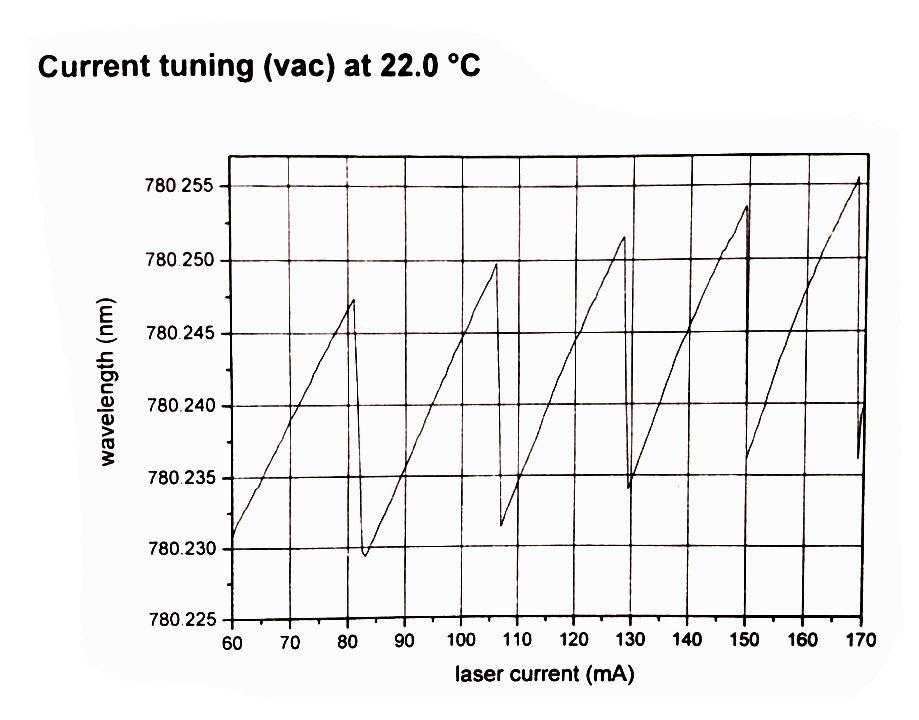
\includegraphics[scale = 0.4]{currentTuning.jpg}
    \captionof{figure}{Currunt Tuning at \SI{22}{\celsius} from laser instructions}
    \label{image:currentTuning}
\end{center}